\subsection{Ein expandierendes Universum}
\begin{itemize}
	\item Betrachte eine homogene Kugel der Massendichte $\rho=\rho(t)$
	\item Ort eines Volumenelements:
		\begin{equation*}
			\vec{r}(t)=\underset{\underset{\underset{a(t_0)=1, t_0\hat{=}\text{heute}}{\text{Skalenfaktor}}}{\uparrow}}{a(t)}\vec{r}(t_0)
		\end{equation*}
		\begin{itemize}
			\item Position eines mitbewegten Beobachters mit Weltlinie $\left(\vec{r},t\right)=\left(a(t)\cdot \vec{r}_0,t\right)$ und Geschwindigkeit
				\begin{equation*}
					\vec{v}=\frac{d}{dt}\vec{r}=\frac{da}{dt}\cdot\vec{r}_0=\frac{\dot{a}}{a}\cdot\vec{r}(t)=:H(t)\cdot\vec{r}(t)
				\end{equation*}
				$\leadsto$ Expansionsrate: $H(t):=\frac{\dot{a}}{a}$
		\end{itemize}
	\item insbesondere Relativgeschwindigkeit zweier mitbewegter Punkte:
		\begin{equation*}
			\Delta\vec{v}=\vec{c}\left(\vec{r}+\Delta\vec{r},t\right)-\vec{v}\left(\vec{r},t\right)=H(t)\cdot\Delta\vec{r}
		\end{equation*}
		$\hat{=}$ Verallgemeinerung des Hubble-Gesetzes, für das gilt: $H(t_0)=H_0$
\end{itemize}
\subsubsection{Newtonsche Kosmologie}
\begin{itemize}
	\item Radius $\vec{r}(t)\equiv a(t)r$ einer Kugel der Masse:
		\begin{equation*}
			M(r_0)=\frac{4\pi}{3}\rho_0r_0^3=\frac{4\pi}{3}\rho(t)\big(a(t)\cdot r_0\big)^3
		\end{equation*}
		\begin{itemize}
			\item $\rho(t)=\rho_0\cdot a(t)^{-3}$
		\end{itemize}
	\item Bewegungsgleichung:
		\begin{align*}
			\ddot{r(t)}&=-\frac{G\cdot M(r_0)}{r^2}=-\frac{4\pi G}{3}\frac{\rho_0\cdot r_0^3}{r^2}\\
			\ddot{a}&=\frac{\ddot{r}}{r}=-\frac{4\pi G}{3}\rho\cdot a\qquad\text{unabhängig von $r_0$}
		\end{align*}
	\item "`Energieerhaltung"':
		\begin{align*}
			\dot{a}^2&=\frac{8\pi G}{3}\rho_0\frac{1}{a}-K\cdot c^2\\
			&=\frac{8\pi G}{3}\rho(t)\cdot a(t)-Kc^2
		\end{align*}
		mit $K\propto $ Gesamtenergie eines mitbewegten Teilchens
		\begin{itemize}[label={$\cdot$}]
			\item wenn $K<0\Rightarrow \dot{a}>0\Rightarrow$ Universum expandiert ewig
			\item wenn $K>0\Rightarrow \dot{a}<0\Rightarrow$ bei größeren $t\Rightarrow$ Universum rekollabiert
			\item wenn $K=0\Rightarrow$ kritische Dichte:
				\begin{equation*}
					\left(\frac{\dot{a}(t_0)}{a(t_0)}\right)^2=\frac{8\pi G}{3}\rho_0
				\end{equation*}
		\end{itemize}
		\begin{itemize}
			\item $\rho_c=\frac{3H_0^2}{8\pi G}\approx\SI{1.88e-29}{h^2\frac{\g}{\cm^3}}$
			\item Dichteparameter: $\Omega_0:=\frac{\rho_0}{\rho_c}$
		\end{itemize}
\end{itemize}
\subsubsection{Relativitätstheorie}
\begin{itemize}
	\item \textbf{Relativitätsprinzip} (Einstein 1905):\\
		Die Naturgesetze haben in allen Inertialsystemen die selbe Form.
	\item betrifft Wechsel zwischen Bezugssystemen mit konstanter Relativgeschwindigkeit ($\Rightarrow$ spezielle Lorentz-Transformation)
	\item daraus folgende Vorhersagen wurden spektakulär nachgewiesen (Längenkontraktion, Zeitdilatation, etc.) und betrifft alle Untergebiete der modernen Physik
	\item Für die Kosmologie muss die Gravitation miteinbezogen werden, da es die einzige \textbf{bekannte} Kraft ist, die auf kosmischen Distanzen wirkt
	\item \textbf{Äquivalenzprinzip} (Einstein 1914):\\
		In jedem Punkt der Raumzeit (mit und ohne Gravitationsfelder) kann man ein (in Zeit und Raum) \textbf{lokales} Inertialsystem so wählen, dass die physikalischen Gesetze denen eines unbeschleunigten kartesischen Bezugssystems entsprechen
	\item Mathematisch kann gezeigt werden, dass die Gravitation die Geometrie der Raumzeit beeinflusst
		\begin{enumerate}[label={$(\roman*)$}]
			\item \textbf{ohne} Gravitation:
				\begin{equation*}
					ds^2=c^2dt^2-dx^2-dy^2-dz^2
				\end{equation*}
			\item \textbf{mit} Gravitation:
				\begin{equation*}
					ds^2=\sum\limits_{\mu,\nu=0}^3g_{\mu\nu}dx^\mu dx^\nu \qquad \text{ mit } x^\mu=(c\cdot t, x, y, z)
				\end{equation*}
		\end{enumerate}
	\item Der metrische Tensor $g_{\mu\nu}=g_{\nu\mu}$ bestimmt die geometrischen Eigenschaften der Raumzeit
	\item $g_{\mu\nu}$ ergibt sich aus den Einstein'schen Feldgleichungen der Allgemeinen Relativitätstheorie $\rightarrow$ $\num{10}$ nichtlineare, partielle, gekoppelte Differentialgleichungen für die $\num{10}$ unabhängigen Komponenten der Metrik
		\begin{equation*}
			\underset{\underset{\underset{\underset{\text{ihre 1. und 2. Ableitungen}}{\text{enthält $g_{\mu\nu}$ und}}}{\text{Einstein-Tensor}}}{\uparrow}}{G_{\mu\nu}}=\underset{\kappa=\frac{8\pi G}{c^4}\ \left[\text{SI}\right]}{\underset{\underset{\underset{\underset{\underset{\text{Einheitensystem)}}{\text{dem gewählten}}}{\text{(ergibt sich aus}}}{\text{Konstante}}}{\uparrow}}{\kappa}}\cdot \underset{\underset{\text{Energieimpulstensor}}{\uparrow}}{T_{\mu\nu}}
		\end{equation*}
		\begin{align*}
			G_{\mu\nu}&=R_{\mu\nu}-\frac{1}{2}g_{\mu\nu}R\\
			R_{\mu\nu}&=\sum\limits_{\alpha=0}^3R^\alpha_{\mu\alpha\nu} \qquad R=\sum\limits_{\mu,\nu=0}^3g^{\mu\nu}R_{\mu\nu}\\
			R_{\nu\sigma\tau}^\mu&=\partial_\sigma \Gamma^\mu_{\nu\tau}-\partial_\tau \Gamma^\mu_\nu\sigma + \sum\limits_{\alpha=0}^3\Gamma^\mu_{\sigma\alpha}\Gamma^\alpha_{\nu\tau}-\sum\limits_{\alpha=0}^3\Gamma^\mu_{\tau\alpha}\Gamma^\alpha_{\mu\sigma}\\
			\Gamma^\sigma_{\mu\nu}&=\sum\limits_{\alpha=0}^3\frac{1}{2}g^{\sigma\alpha}\left(\partial_\nu g_{\alpha\mu}+\partial_\mu g_{\alpha\nu}-\partial_\alpha g_{\mu\nu}\right)
		\end{align*}
\end{itemize}
\subsubsection{Gekrümmte Räume}
\begin{itemize}
	\item Die Ebene ist flach, Vektoren können parallel verschoben werden, ohne dass sie ihre Richtung ändern
		\begin{figure}[H]
			\centering
			\begin{tikzpicture}
				\draw[->,>=stealth] (0,0)node[below left]{$\vec{u}$}--(0,2)node[midway,name=x]{};
				\draw[->,>=stealth] (2,0)node[below right]{$\vec{u}'$}--(2,2)node[midway,name=y]{};
				\draw[->,densely dashed,shorten <= 2pt, shorten >= 2pt] (x)--(y);
			\end{tikzpicture}
		\end{figure}
	\item Ist die Kugel flach?
		\begin{figure}[H]
			\begin{multicols}{2}
				\begin{figure}[H]
					\centering
					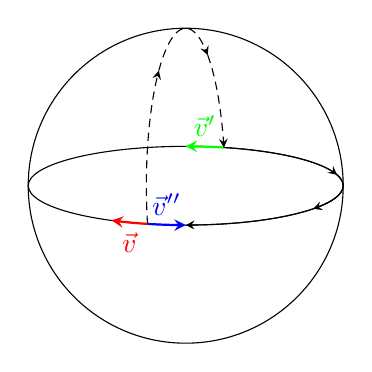
\begin{tikzpicture}[>=stealth]
						\draw (0,0)circle(2cm);
						\draw (0,0)ellipse(2cm and 0.5cm);
						\draw[densely dashed,->,domain=194:133] plot({0.5*cos(\x)},{2*sin(\x)});
						\draw[densely dashed,->,domain=133:56] plot({0.5*cos(\x)},{2*sin(\x)});
						\draw[green,->,domain=76:90,thick] plot({2*cos(\x)},{0.5*sin(\x)});
						\node[green,above] at ({2*cos(83)},{0.5*sin(83)}){$\vec{v}'$};
						\draw[densely dashed,->,domain=56:14] plot({0.5*cos(\x)},{2*sin(\x)});
						\draw[->,domain=76:16] plot({2*cos(\x)},{0.5*sin(\x)});
						\draw[->,domain=16:-36] plot({2*cos(\x)},{0.5*sin(\x)});
						\draw[->,domain=16:-90] plot({2*cos(\x)},{0.5*sin(\x)});
						\draw[red,->,domain=256:242,thick] plot({2*cos(\x)},{0.5*sin(\x)});
						\node[red,below] at ({2*cos(249)},{0.5*sin(249)}){$\vec{v}$};
						\draw[blue,->,domain=256:270,thick] plot({2*cos(\x)},{0.5*sin(\x)});
						\node[blue,above] at ({2*cos(263)},{0.5*sin(263)}){$\vec{v}''$};
					\end{tikzpicture}
				\end{figure}\columnbreak
				Parallelverschiebung von $\vec{v}$ liefert nach Abschluss des gestrichelten Weges den Vektor $\vec{v}'$ und dann mit Verschiebung entlang des Äquators den Vektor $\vec{v}''=-\vec{v}$
			\end{multicols}
		\end{figure}
	\item Weitere Beispiele:
		\begin{figure}[H]
			\centering
			\begin{multicols}{3}
				\begin{figure}[H]
					\centering
					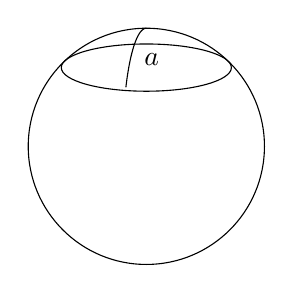
\begin{tikzpicture}
						\draw (0,0)circle(1.5cm);
						\draw (0,1)ellipse(1.08cm and 0.3cm);
						\draw[domain=90:150] plot({0.3*cos(\x)},{1.5*sin(\x)});
						\node[below right] at ({0.3*cos(120)},{1.5*sin(120)}){$a$};
					\end{tikzpicture}\vspace{0.2cm}\\
					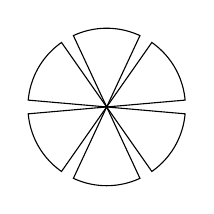
\begin{tikzpicture}
						\foreach \y in {0,...,5}{
							\draw[domain={\y*60+5}:{(\y+1)*60-5}] (0,0)--plot({cos(\x)},{sin(\x)})--(0,0);
						}
					\end{tikzpicture}
				\end{figure}
				$C<2\pi a$
				\columnbreak
				\begin{figure}[H]
					\centering
					\begin{tikzpicture}[scale=0.7]
						\draw (-3,-2)rectangle(3,2);
						\draw (0,0)circle(1cm);
					\end{tikzpicture}\vspace{0.2cm}\\
					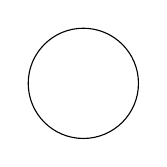
\begin{tikzpicture}[scale=0.7]
						\draw (0,0)circle(1cm);
					\end{tikzpicture}
				\end{figure}
				$C=2\pi a$\\\columnbreak
			\end{multicols}
		\end{figure}
	\item Wie kann man Krümmung messen?\\
	$to$ Vergleich von Kreisumfang $C$ und Kreisfläche $A$ eines Kreises mit Radius $a$
		\begin{table}[H]
			\begin{tabular}{l|c|c|r}
				\hline Kugel & $C<2\pi a$ & $A<\pi a^2$ & positiv\\
				\hline Ebene & $C=2\pi a$ & $A=\pi a^2$ & null (=flach)\\
				\hline Sattel & $C>2\pi a$ & $A>\pi a^2$ & negativ \\\hline
			\end{tabular}
		\end{table}
		\noindent\textbf{Krümmung ist eine intrinsische Eigenschaft!}\\
		d.h. man kann nie messen, ohne den \glqq Raum\grqq{} zu verlassen (essentiell in der Kosmologie)
\end{itemize}
\subsubsection{Modifikation der Newtonschen Kosmologie}
\begin{enumerate}[label={$(\alph*)$}]
	\item Äquivalenz von Masse und Energie ($E=mc^2$)
		\begin{itemize}[label={$\Rightarrow$}]
			\item $\rho$ in den kosmologischen Bewegungsgleichungen enthält nicht nur die Materiedichte
		\end{itemize}
	\item Die Einsteinschen Feldgleichungen der ART erlauben einen zusätzlichen Term, die \textbf{Kosmologische Konstante $\Lambda$}
	\item Die Interpretatino der Expansion des Kosmos ändert sich: Das Universum ist keine expandierende Kugel, sondern der \textbf{Raum selbst expandiert}
		\begin{itemize}[label={$\Rightarrow$}]
			\item Die Rotverschiebung ist eine Eigenschaft der expandierenden Raumzeit ($a=a(t)=\text{Skalenfaktor}$)
		\end{itemize}
\end{enumerate}
\begin{itemize}
	\item \textbf{Erster Hauptsatz der Thermodynamik}\\
		\begin{equation*}
			\underset{\underset{\underset{\text{inneren Energie}}{\text{Änderung der}}}{\uparrow}}{dU}=-\underset{\underset{\text{Druck}}{\uparrow}}{P}\cdot\underset{\underset{\underset{\text{Volumenänderung}}{\text{(adiabatische)}}}{\uparrow}}{dV}
		\end{equation*}
		Aus den Gleichungen der Allgemeinen Relativitätstheorie folgt eine analoge Relation für einen homogenen und isotropen Kosmos:
		\begin{equation*}
			\frac{d}{dt}(\underset{\underset{\text{Energiedichte}}{\downarrow}}{\underbrace{c^2\rho}}a^3)=-P\cdot\frac{d(a^3)}{dt}
		\end{equation*}
		(d.h. für "`normale"' Materie ist $\rho$ die Massendichte, $P$ der Druck der Materie und $V=a^3(t)\cdot V_0$ das Volumen)
	\item Die Friedmann-Lena\^itre Expansionsgleichung:
		\begin{align*}
			\left(\frac{\dot{a}}{a}\right)^2&=\frac{8\pi G}{3}\rho -\frac{Kc^2}{a^2}+\frac{\Lambda}{3} \qquad (F1)\\
			\frac{\ddot{a}}{a}&=-\frac{4\pi G}{3}\left(\rho+\frac{3P}{c^2}\right)+\frac{1}{3} \qquad (F2)
		\end{align*}
		$\cdot$  Unterschiede zu Newton:
		\begin{enumerate}[label={$(\roman*)$}]
			\item zusätzlicher Druckterm um (F2)
			\item kosmologische Konstante
		\end{enumerate}
	\item Die \textbf{Kosmologische Konstante}:
		NB: Falls $\Lambda =0$, gibt es keine Lösung der Friedmann-Lena\^itre-Gleichungen mit $\dot{a}=0$ (siehe Übungsblatt 7, Aufgabe 2)
		\begin{itemize}
			\item $\Lambda\neq 0$ eingeführt von Einstein um das statische Universum "zu retten"
			\item[1923] Eddington diskutiert die Möglichkeit eines nicht statischen Universums
			\item[1929] Hubble beobachtet eine systematische Expansion\\
				Quantenfeldtheorie: auch das Vakuum enthält eine nicht verschwindende Energie
			\item mathematisch äquivalent zu $\Lambda\neq 0$ (aber Größenordungen stimmen nicht!)
		\end{itemize}
\end{itemize}
\subsubsection{Die Materiekomponenten des Universums}
\begin{itemize}
	\item Druckfreie Materie ("`Staub"')
		\begin{equation*}
			P_m=0
		\end{equation*}
		Druck eines Gases $\propto$ thermische Bewegung\\
		z.B. Moleküle der Luft mit $v\sim v_{\text{Schall}}\sim\SI{300}{\frac{\m}{\s}}\ \Rightarrow P_m<<\rho_mc^2$
	\item Strahlung $P_r=\frac{1}{3}\rho_rc^2$\\
		z.B. Photonen des CMB
	\item Vakuumenergie
		\begin{equation*}
			P_V=-\underset{\underset{\underset{\text{mit $\rho_V=cnst.$}}{\text{aus dem 1. HS (s.o.)}}}{\uparrow}}{\rho_V}c^2
		\end{equation*}
		Das Vakuum übt einen negativen Druck aus
\end{itemize}
\subsubsection{Heuristische Herleitung der Friedmann-Lena\^itre-Expansionsgleichungen}
\underline{IVB}: Eine korrekte Herleitung ergibt sich direkt aus der ART!
\begin{itemize}
	\item Hier nutzen wir die Newtonschen Gleichungen und reinterpretieren die "`Energieerhaltung"'
		\begin{equation*}
			\dot{a}^2=\frac{8\pi G}{3}{\rho}a^2-Kc^2\overset{\frac{d}{dt}}{\Rightarrow} 2\dot{a}\ddot{a}=\frac{8\pi G}{3}\left(\dot{\rho}a^3+2\rho a\dot{a}\right)
		\end{equation*}
	\item 1. HS $\left(\frac{d}{dt}\left(c^2\rho a^3\right)=-P\frac{d(a^3)}{dt}\right)$\\
		\begin{align*}
			\dot{\rho}a^3+3\rho a^2\dot{a}&=-3\frac{P}{c^2}a^2\dot{a}\\
			\Rightarrow \dot{\rho}&=-3\rho\frac{\dot{a}}{a}-3\frac{P}{c^2}\frac{\dot{a}}{a} \quad \text{ und einsetzen ergibt:}\\
			\Rightarrow \dot{a}\ddot{a}&=\frac{4\pi G}{3}\left(-\rho\dot{a}a-3\frac{P}{c^2}\dot{a} a\right)
			\Rightarrow \frac{\ddot{a}}{a}&=-\frac{4\pi G}{3}\left(\rho+\frac{3P}{c^2}\right)
		\end{align*}
	\item neu dabei:
		\begin{align*}
			\rho&=\underset{\underset{\text{Materie}}{\uparrow}}{\rho_m}+\underset{\underset{\underset{\text{(Photonen)}}{\text{Strahlung}}}{\uparrow}}{\rho_r}+\underset{\underset{\text{Vakuum}}{\uparrow}}{\rho_V}\\
			P&=\underset{\underset{\text{Materie}}{\uparrow}}{\sigma}+\underset{\underset{\underset{\text{(Photonen)}}{\text{Strahlung}}}{\uparrow}}{P_r}+\underset{\underset{\text{Vakuum}}{\uparrow}}{P_V}
		\end{align*}
		Schreibe $\rho_V=\frac{1}{8\pi G}$ und $\rho=\rho_m+\rho_r, P=P_R P_V=-\rho_Vc^2$
		\begin{align*}
			\Rightarrow \frac{\ddot{a}}{a}&=-\frac{4\pi G}{3}\left(\rho+\frac{3P}{c^2}+\frac{\Lambda}{8\pi G}-\frac{3}{c^2}\left(\frac{\Lambda}{8\pi G}\right)\cdot c^2\right)\\
			&=-\frac{4\pi G}{3}\left(\rho + \frac{3P}{c^2}\right)+\frac{\Lambda}{3}
		\end{align*}
	\item Und schließlich in der Energieerhaltung:
		\begin{align*}
			\left(\frac{\dot{a}}{a}\right)^2&=\frac{8\pi G}{3}\left(\rho_m+\rho_r+\frac{\Lambda}{8\pi G}\right)-\frac{Kc^2}{a^2}\\
			&=\frac{8\pi G}{3}\rho-\frac{Kc^2}{a^2}+\frac{\Lambda}{3} \Rightarrow \text{(F1) und (F2)} \square
		\end{align*}
		N.B: Wert von $\Lambda$ lässt sich bisher nicht aus mikroskopischen Theorien herleiten.
		\begin{itemize}
			\item Eines der großen Rätsel der heutigen Physik
		\end{itemize}
\end{itemize}
\subsubsection{Diskussion der Expansionsgleichungen}
\begin{itemize}
	\item Entwicklung der kosmischen Dichte (folgt aus dem 1. Hauptsatz)
		\begin{itemize}[label={$\cdot$}]
			\item "`Staub"': $P_m=0\Rightarrow \rho_m(t)\sim a(t)^{-3}$
			\item "`Strahlung"': $P_r=\frac{1}{3}\rho_rc^2\Rightarrow \frac{d}{dt}\left(\rho_ra^3\right)=-\frac{1}{3}\rho_r\frac{da^3}{dt}$
				\begin{equation*}
					\dot{rho}_ra^3=-4a^2\dot{a}\rho_r \Rightarrow \frac{\dot{\rho}_r}{\rho_r}=-4\frac{\dot{a}}{a}\Rightarrow \rho_r(t)\sim a(t)^{-4}
				\end{equation*}
				Vakuum: $\rho_V=cnst.$\\
				\begin{equation*}
					\Rightarrow \rho_m(t)=\rho_{m,0}a(t)^{-3},\rho_r(t)=\rho_{r,0}a^{-4}(t),\rho_V(t)=\rho_V
				\end{equation*}
		\end{itemize}
	\item Grund für $\rho_r\sim a^{-4}$: Nicht nur die Anzahldichte der Photonen nimmt ab (mit $a^{-3}(t)$), sondern auch ihre Energie (Rotverschiebung)
		\begin{equation*}
			E=h\cdot\nu = h\cdot\frac{c}{\lambda}\qquad\text{ mit }\qquad\lambda\sim a(t)\Rightarrow \rho_r(t)\sim a^{-3}(t)\cdot a^{-1}(t)=a^{-4}(t)
		\end{equation*}
\end{itemize}
